\chapter{Background \& Theory}
  \section{Databases for AU estimation}
    The following datasets contain AU labels of subjects which are relevant to this work:

    \begin{itemize}
        \item The DISFA database \cite{disfa}, which contains 27 subjects whose spontaneous
              facial expressions were captured in controlled recording conditions. Further information is found in section \ref{disfa_list}.
    % Participants were instructed by an experimenter to perform a series of 23 facial displays; these included single action units and combinations of action units
        \item CK+ \cite{Lucey2010} containing 123 subjects recorded with faces in strictly frontal positions. The subjects were asked to perform a set of
              23 facial displays some of which represented single AUs and others combiniations of AUs. Each display lasted between 9-60 frames
              and the image resolution is $640\times 490$.
        \item FERA 2015 BP4D-Spontaneous Dataset \cite{Valstar}:
              containing 41 subjects and 34 AUs, the subjects were young adults who
              spontaneously generated emotional responses to stimulus tasks.
    \end{itemize}

    This is just a small selection, however it is representative of the types of
    datasets available. Each frame of the videos has a label which describes which AUs are
    present and their intensity. Hence two distinct problems can be tackled here, intensity
    estimation and classification, this work follows the classification route however
    with neural networks it is potentially not a radically different problem.

    Larger datasets, without AU labels also exist such as the Toronoto Face Dataset\cite{tfd}
    or SEMAINE \cite{semaine}, these are relevant to possible extensions of this project as their
    images could be included in the unsupervised learning stages of the proposed model. This also
    applies to CK+ and FERA 2015, but potentially learning from these larger datasets would
    be more effective.

    % A key challenge with these datasets is that they often have very unbalanced and
    % sparse labels as shown in figure \ref{disfastats}. This calls for methods
    % to balance training samples with respect to this imbalance and is the
    % motivation for using some unsupervised learning techniques, in order to extract information
    % from the unlabelled data.


    % However, in our case, all data is labelled.
    % you could explain that successful autoencoder training might show a direction to make use of large datatsets without AU annotations (like TFD)



    % A further two datasets are the TFD and SEMAINE, these do not contain AUs but often crop up in the
    % literature:
    % \begin{itemize}
    %      \item TFD \cite{tfd} Toronto Face Dataset
    %      \item The SEMAINE \cite{semaine} corpus which contains recordings
    %            of people interacting with a Sensitive Artificial Listener (SAL) in controlled conditions.
    % \end{itemize}

    \section{The DISFA dataset} \label{disfa_list}
    The Denver Intensity of Spontaneous Facial Action (DISFA)\cite{disfa} is of
    of central interest to the project, it is a set
    of videos of people watching 9 short clips from youtube which try to span a range
    of emotions such as emotions happiness, surprise, fear, disgust and sadness. Included
    are 27 subjects with 12 AUs.

    Each frame in each subject video has a label which quantifies how much of each
    AU is present on a scale of 0-5, the distribution of intensities is shown in table \ref{compau}.

    A challenge of the DISFA dataset is that it has many frames which are neutral, this is shown
    per subject in figure \ref{disfastats}. Many of the subjects have over 40\% of their frames as neutral expressions
    , one outlier has over 75\% such expressions.

    \begin{table}[h!]
    \centering

    \begin{tabular}{lllllll}
    \hline
    Intensity & 0      & 1     & 2     & 3     & 4    & 5    \\ \hline
    AU1       & 112286 & 2272  & 1749  & 2809  & 1393 & 555  \\
    AU2       & 99165  & 1720  & 934   & 3505  & 836  & 369  \\
    AU4       & 106160 & 4661  & 7636  & 6586  & 4328 & 1383 \\
    AU5       & 99015  & 1579  & 719   & 293   & 104  & 34   \\
    AU6       & 106425 & 9157  & 5986  & 3599  & 601  & 141  \\
    AU9       & 99458  & 1659  & 2035  & 3045  & 316  & 77   \\
    AU12      & 99987  & 13943 & 6869  & 7233  & 2550 & 172  \\
    AU15      & 108358 & 5180  & 1618  & 1017  & 47   & 0    \\
    AU17      & 117824 & 6342  & 4184  & 2281  & 112  & 11   \\
    AU20      & 121377 & 1591  & 1608  & 1305  & 28   & 0    \\
    AU25      & 84721  & 9805  & 13935 & 15674 & 5580 & 1039 \\
    AU26      & 105778 & 13443 & 7473  & 3529  & 314  & 217  \\ \hline
    \end{tabular}
    \caption{A comparison of the number of occurrences of each intensity for each AU in the DISFA dataset. Note the total number
    of AUs tabled here is larger than the number of frames, this is because some frames have multiple AUs present.} \label{compau}
    \end{table}


    \begin{figure}[h!]
      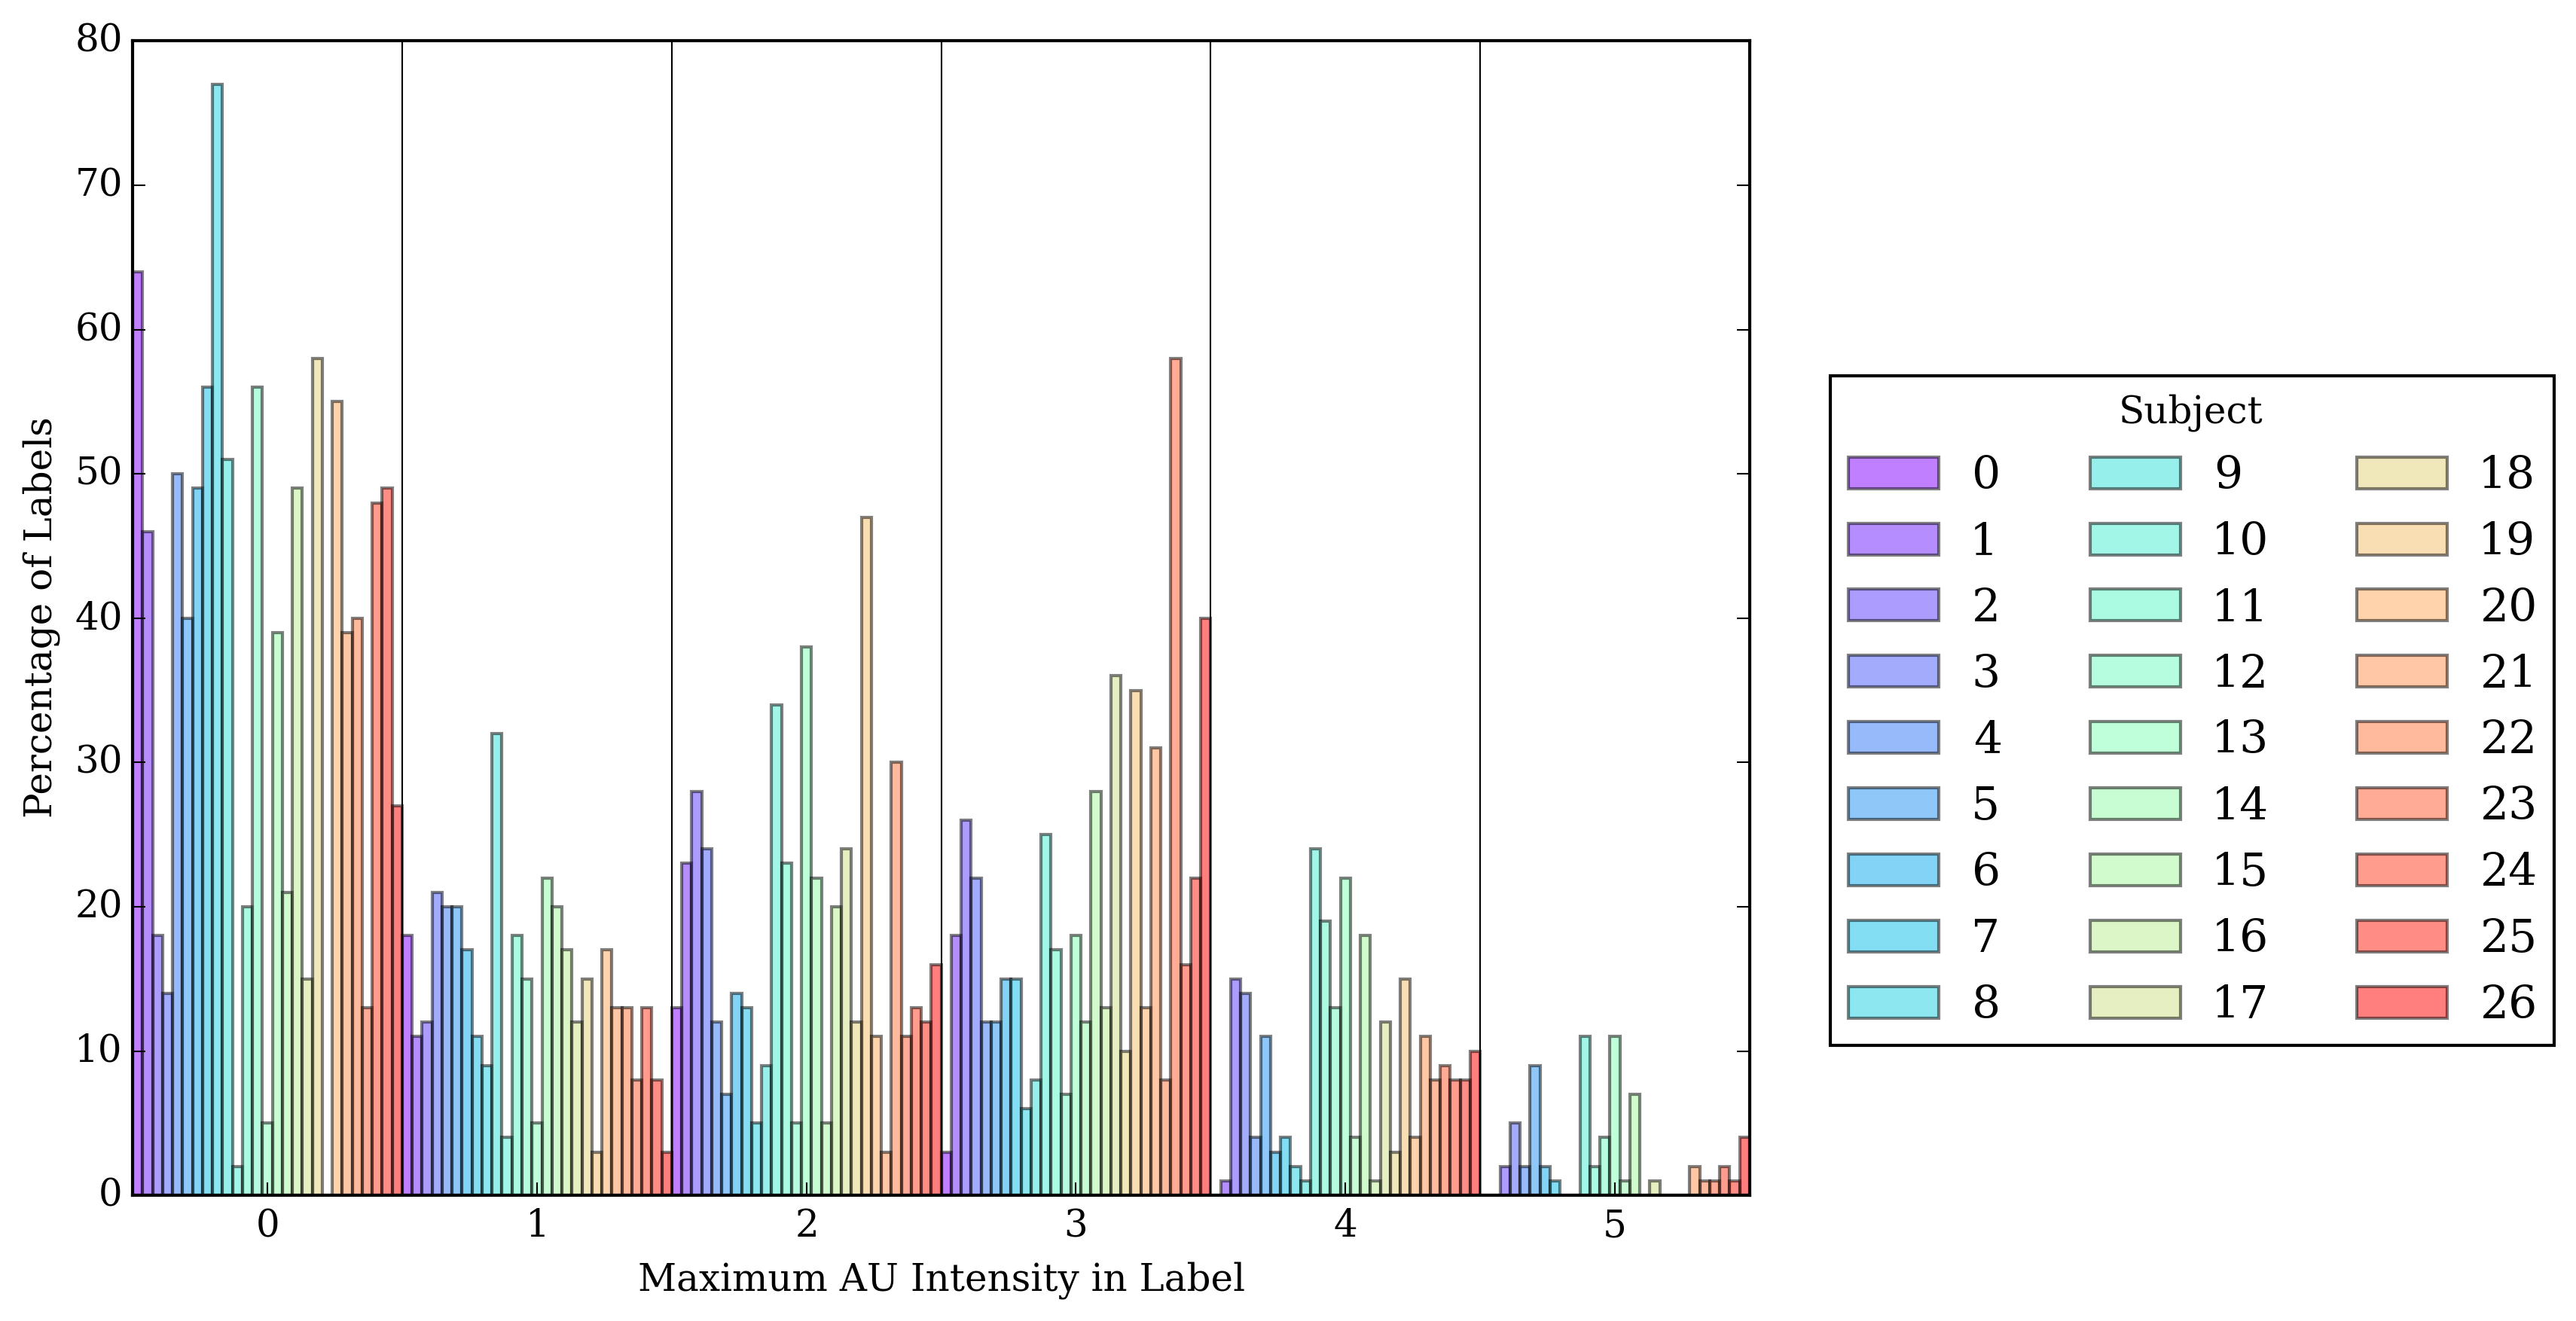
\includegraphics[width=\textwidth]{../graphs/maximum_label_intensity_disfa.pdf}
      \caption{This graph shows what the maximum value in each label is in the DISFA dataset per subject. This
      is done to illustrate the number of labels which contain very little information
      and pose an issue for a typical neural network structure. It also shows that there
      is quite a large degree of variation between subjects. In this work, frames are often referred to as neutral
      in the figure these are all the labels with maximum intensity zero.}\label{disfastats}
    \end{figure}

\section{Deep Learning \& Neural Networks}
  Deep learning algorithms have recently been applied to image classification
  and object detection tasks with lots of success. \cite{Girshick2014,Krizhevsky2012}
  Three main factors have been instrumental in making this happen \cite{Jaiswal2016}:
  \begin{itemize}
    \item Efficient methods to train deep artificial neural networks
    \item Improved parallel processing hardware such as GPU's
    \item An abundance of labelled data
  \end{itemize}
  This development has moved the focus of classification tasks away from feature engineering,
  which seeks to manually find general methods of quantifying and locating features in image data, to
  architecture design \cite{StephenMerity2016}, where the primary concern is the structure and size of the neural network that has to
  learn the desired task.

  The following section explains the key components that a deep learning algorithm requires,
  derivations of gradients for back propagation are left out as the focus of the project is to
  see how these components can interact and be built up and such derivations would add little to the understanding,
  for a detailed analysis see \cite{Bishop1995}.

  \subsection{Artificial Neural Networks} \label{sec:anns}
    An artificial neuron is a function which takes in a vector of inputs, computes their
    weighted sum and applies a non-linearity as follows:
    \begin{equation}
      a(\mathbf{x}) = \sigma \left ( \sum_{i=1}^N w_ix_i + b \right )
    \end{equation}
    Here $\sigma$ is a scalar function, $w_i$ is a scalar weight and $b$ is its bias. $N$ is the size of the input and weight vector.
    These neurons can be combined into layered networks to construct artificial neural networks.
    The weights $w$ can then be rewritten as matrices $\mathbf{W}$ which define how
    activations from one layer are transferred to the next\footnote{Note: in this report when a vector
    is put into a scalar function it is assumed that it acts on each element of
    the vector. The only exception is with the softmax.}.
    \begin{equation}
      \mathbf{a}(\mathbf{x}) = \mathbf{\sigma} \left ( \mathbf{W}\mathbf{x} + \mathbf{b} \right ) \label{eq:softmax}
    \end{equation}

    If all of the variables in $\mathbf{W}$ are trainable then this is reffered to as a
    fully connected layer.

    Popular activation functions include:
    \begin{multicols}{2}


      \begin{equation}
        \text{The sigmoid:}\quad
        \sigma (x) = \frac{1}{1-e^{-x}} \label{eq:sigmoid}
      \end{equation}


      \begin{equation}
        \text{ReLU:}\quad
        \sigma(x) = \max(0,x)
      \end{equation}

      \begin{equation}
        \text{Leaky ReLU:}\quad
        \sigma(x) = \max(\alpha x,x)
      \end{equation}


      \begin{equation}
        \text{Hyperbolic tan:}\quad
        \sigma(x)=\frac{e^x - e^{-x}}{e^x + e^{-x}}
      \end{equation}


      \begin{equation}
        \text{The softmax:}\quad
        \sigma(\mathbf{x})_j = \frac{e^{x_j}}{\sum_i e^{x_i}}
      \end{equation}


    \end{multicols}

    For the leaky ReLU $\alpha$ is some small constant, the purpose is to allow gradients to carry on
    propagating if activations fall below zero. This approach has been proven to improve performance in some classification
    tasks \cite{Xu2015}.

    \begin{figure} \label{disfagraph}
      \center
      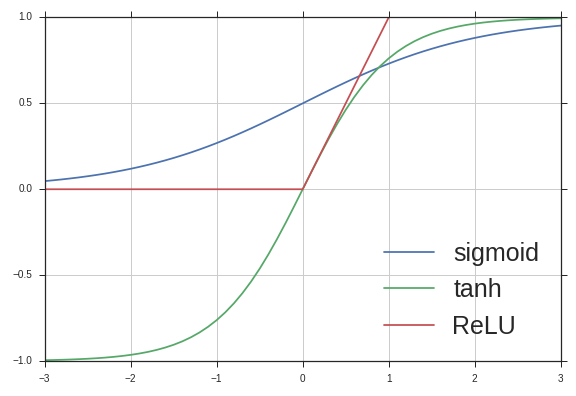
\includegraphics[width=.5\textwidth]{../graphs/actfuncs.pdf}
      \caption{Comparison of common activation functions for neural networks}
    \end{figure}



    An $N$ layer network can then be thought of as a function with a nested:
    \begin{equation} \label{eq:ynn}
      \mathbf{y} = \mathbf{a}_{N}(\mathbf{a}_{l-1}(...\mathbf{a}_1(\mathbf{x})...))
    \end{equation}
    Now assuming there exists a set of $\tilde{\mathbf{x}}$ and $\tilde{\mathbf{y}}$ which make
    up a training data set, these could be sets of images and labels, then a cost function
    to optimise can be defined:
    \begin{equation}
      J(\tilde{\mathbf{x}},\tilde{\mathbf{y}},\mathbf{y}) = \frac{1}{N}\left |\mathbf{y}(\tilde{\mathbf{x}})-\tilde{\mathbf{y}}\right | ^2
    \end{equation}
    This is called the mean squared error, here $\tilde{\mathbf{x}}$ and $\tilde{\mathbf{y}}$ could
    be the images and labels of a dataset respectively and $\mathbf{y}$ represents the network we are evaluating (equation \ref{eq:ynn}). Another popular cost function is
    the cross entropy:
    \begin{equation}
      J(\tilde{\mathbf{x}},\tilde{\mathbf{y}},\mathbf{y}) = -\frac{1}{N}\tilde{\mathbf{y}}\cdot\log(\mathbf{y}(\tilde{\mathbf{x}}))
    \end{equation}

    This has the property of giving high costs when a positive example is incorrectly classified as negative: $\lim _{y\rightarrow0}\frac{1}{N}1\cdot \log(y) = \infty$
    and not adjusting the weights otherwise.

  \subsection{Training}
      This report will often refer to the process of training, the objective of training is to find
      a $\tilde{\mathbf{y}}^* \in \mathbf{Y}$ that satisfies the following definition:

      \begin{equation}
        J(\tilde{\mathbf{x}},\tilde{\mathbf{y}},\mathbf{y}^*) \leq J(\tilde{\mathbf{x}},\tilde{\mathbf{y}},\mathbf{y}) \quad \forall \mathbf{y} \in \mathbf{Y}
      \end{equation}

      Where $\mathbf{Y}$ is defined as the set of all possible $\mathbf{y}$ functions which are constructed with a series $\mathbf{W}$ and $\mathbf{b}$ matrices as defined in the previous section.
      As $J$ cannot be known fully and is unlikely to be convex \footnote{Which would guarantee a global minimum, for example a parabola $y(x)=x^2$ is convex and has a minimum at $y(0)$}
      , this goal is impracticable to achieve in practice.
      Training is therefore the process of finding a local minimum by taking a path through $J$ by varying
      the function $ \mathbf{y} $, the different strategies by which $J$ is explored are called
      training algorithms or optimizers.

      This is actualised by taking the derivative, with respect to each weight variable
      in the network, $i$ and updating those variables in order to reduce $J$:

      \begin{equation}
        w_i \leftarrow w_i - \eta \frac{\partial J }{\partial w_{i}}(\tilde{\mathbf{x}},\tilde{\mathbf{y}},\mathbf{y})
      \end{equation}

      This occurs for every $i$ where $w_i$ is some trainable variable in $\mathbf{y}$.
      This is the simplest way to achieve training or gradient descent, this is referred to as backpropagation
      because computing the derivative requires the repeated use of the chain rule.
      Advanced versions of this are used in the project, in particular the Adam algorithm
      which is descried in \cite{adam}.

      %
      % The derivative of these cost functions with respect to each weight and bias variable
      % in the network is then calculated.
      % The simplest way is to do this is per training example, however stochastic gradient
      % descent\cite{Amari1993} has emerged as a superior method. Simply put it computes the average gradient with respect
      % to many randomly drawn samples, it has the advantage of following a smoother path
      % towards the local minimum. Another training algorithm which builds on this is called is Adam \cite{adam}.
      % http://sebastianruder.com/optimizing-gradient-descent/index.html#adam
      % \url{https://www.quora.com/Can-you-explain-basic-intuition-behind-ADAM-a-method-for-stochastic-optimization}
  \subsection{Convolutional Layers}
    A convolutional layer is a generalisation of simple fully connected layers described
    above. It consists of a set of $K$ filters of size $m\times m$, which are applied to the input to produce
    a set of $K$ outputs. The filters are applied with a 2D convolution.


    To describe them, firstly assume that any vector described in the previous section
    can also be rewritten as a matrix, i.e $\mathbf{x} \in \mathbb{R}^{n}
    \rightarrow \mathbf{x} \in \mathbb{R}^{N \times M} \quad NM=n$, in practice this is made
    easy by using numbers which factorise well.

    Then the following equation describes the output of a convolutional layer:
    \begin{equation} \label{CNN}
      \mathbf{a}(\mathbf{x})_{ijk} = \sigma \left ( \sum_{a=0}^{m-1}\sum_{b=0}^{m-1}(w_{abk}x_{(i+a)(j+b)k}) + b_k \right )
    \end{equation}
    Here $i,j$  denote row, column indices for the matrix (image) $\mathbf{x}$, $k$ is the filter index, $w_{abk}$
    gives the filter element and $b_k$ is the bias for that filter. This is done for all $K$ filters.

    One issue is how to deal with indices which are out of bounds, SAME padding can be used which sets out of bounds
    elements to zero and so preserves the image size or VALID can be used, this keeps the filter within the bounds of the
    image and hence the output is of a smaller dimension. Lastly a stride greater than 1 can be incorporated into equation
    \ref{CNN} meaning that $\mathbf{a}$ is only computed for a fraction of indices $i,j$.
    % \begin{equation}
    % 	C : \mathbb{R}^{n\times m \times p \times l} \rightarrow \mathbb{R}^{N\times M \times l \times K}
    % \end{equation}
    %con%
  \subsection{Max Pooling Layers}
    A max pooling layer simply splits its input into a set of sections and extracts
    the highest value from each. It is a simple but effective method to down sample
    an image, it helps to keep the computational overhead of these algorithms
    down. However a recent trend \cite{Springenberg2015} has emerged where max pooling
    layers are not used, instead a convolutional layer with a large stride accomplishes
    the same amount of down-sampling.
  \subsection{Autoencoders} \label{sec:autoencoders}
    An autoencoder is at its bare minimum a artificial neural network which tries
    to reproduce its input as accurately as possible. So the cost function for the mean squared error becomes:

    \begin{equation} \label{eq:autoencoder_cost}
      J(\tilde{\mathbf{x}},\tilde{\mathbf{y}}) = \frac{1}{N}\left |\mathbf{y}(\tilde{\mathbf{x}})-\tilde{\mathbf{x}}\right | ^2
    \end{equation}

    Constraints are
    placed on the network so that it has to learn to compress the input, the following
    are popular constraints that may be used:
    \begin{itemize}
      \item Few neurons in the hidden layers
      \item Sparsity: the average activation of the neurons can be kept under a
      threshold, typically a small value close to zero \cite{autong}
      \item Noise may be added to the input, this makes the network more likely
      to learn general features.
      \item Weight sharing between encoder and decoder sections. This is possible since
            the encoder and decoders are typically inverses of each other.
    \end{itemize}
    Lastly there are Variational Autoencoders which combine ideas from Bayesian inference
    to create networks which can not only reconstruct their input but also act as a
    distribution which can be sampled from, allowing for the generation of new samples \cite{Kingma2013}.

  \subsection{Joint vs Stacked Autoencoder training}
    A stacked autoencoder is typically used for pre-training a network for a classification task.
    Instead of training the whole structure at once, each layer is trained as the last hidden
    layer of some temporary autoencoder. It has been shown that this can improve classification performance \cite{stacks}.
  \subsection{Convolutional Autoencoder}
    A convolutional autoencoder works in the same way as a standard autoencoder, however
    undoing the max pooling presents a problem, as a max pooling layer throws away
    information, its inverse will never be exact. The following strategies have been
    used with success:
    \begin{itemize}
      \item Replacing each entry with an $n \times n$ matrix filled with the original
      entry.
      \item Replacing each entry with an  $n\times n$  matrix with
      the original entry in the upper left and the other squares set to 0. \cite{Dosovitskiy2015}
    \end{itemize}

    Other than that all other elements have very straightforward inverses and hence
    a convolutional autoencoder can be constructed.
  \subsection{Local Response Normalisation} \label{sec:lrn}
    This section reproduces the local response normalisation proceedure described in \cite{Krizhevsky2012}
    and implemented as the function \texttt{tf.nn.lrn} in TensorFlow.

    It was found to aid generalisation with the ImageNet dataset. The following quote from the paper \cite{Krizhevsky2012}
    describes the motivation for this approach:

    \begin{displayquote}
      This sort of response normalization implements a form of lateral inhibition
      inspired by the type found in real neurons, creating competition for big activities amongst neuron
      outputs computed using different kernels.
    \end{displayquote}

    This is done by normalising over the feature maps which are computed by the different convolutional kernels (or filters).
    The following equation shows the procedure applied to the output of a convolutional layer:

    \begin{equation} \label{eq:lrn}
      \mathbf{a}(\mathbf{x})_{ijk}
      = \mathbf{a}(\mathbf{x})_{ijk}/\left (\rho + \sum^{\min(N-1,i+n/2)}_{m=\max(0,i-n/2)}\mathbf{b}(\mathbf{x})_{ijm} \right )^\beta
    \end{equation}

    the parameter $n$ signifies how many adjacent feature maps to sum over, $N$ is the total number of feature maps.
    Parameters $\rho,n,\alpha$ and $\beta$ are hyperparameters, the values used in \cite{Krizhevsky2012} are
    $k=2,n=5,\alpha=10^{-4}$ and $\beta=0.75$.

  \subsection{Overfitting and Regularisation}
    Unless a machine learning model can learn a truly general hypothesis, it will always perform
    better on the data used to train it than on the data on which it is tested. This is
    called overfitting, this can be avoided by choosing hypotheses which are lie somewhere
    in some ideal region between very simple and very complex.

    Regularisation is the process of constraining or augmenting
    the loss function of a model \cite{Bishop2006} somehow in order to improve its performance.
    Some of these techniques for neural networks are described in this section.
    % http://neuralnetworksanddeeplearning.com/chap3.html#overfitting_and_regularization
    \subsubsection{Denoising}
      For autoencoders, a noise term can be added to the loss function (equation \ref{eq:autoencoder_cost}) as follows:
      \begin{equation} \label{eq:autoencoder_cost_noise}
        J(\tilde{\mathbf{x}},\tilde{\mathbf{y}}) = \frac{1}{N}\left |\mathbf{y}(\tilde{\mathbf{x}}+\mathbf{n})-\tilde{\mathbf{x}}\right | ^2\quad \mathbf{n} \sim \mathbf{\mathcal{N}}(0,\sigma^2)
      \end{equation}
      such noise terms can also be added between the layers of the network. This
      has been shown to improve the number of quality of features learnt by an auteoncoder \cite{stacks,Vincent2008a}.
    \subsubsection{L1 and L2 Regularises} \label{sec:bacl2}
      An additional term can be added to a loss function as follows \cite{Ng2004a}:
      \begin{equation}
        J'(\tilde{\mathbf{x}},\tilde{\mathbf{y}},\mathbf{y}) = J(\tilde{\mathbf{x}},\tilde{\mathbf{y}}) + \beta R(\mathbf{W})
      \end{equation}
      Where $\mathbf{W}$ represents all the weights in $\mathbf{y}$ For L1 Regularisation $R = ||W||_1$ and for L2 $R = ||W||_2^2$.
      This term forces the network to use smaller weights in order to reduce $R$
      and hence reduces the complexity of a model. A simple way to imagine is this
      with a simple model such as a polynomial, $f(x)=\sum_{n=0}^N a_n x^n$, by imposing a
      penalty on the sizes of the $a_n$ terms, simpler polynomials curves will be favoured in
      any training situation.
    \subsubsection{Dropout Layers} \label{sec:dropout}
      Dropout \cite{Srivastava2014} is a technique where neurons on a layer are
      randomly deactivated during training with some probability $p$. This slows overfitting
      as it firstly reduces the number of parameters available in each training step and secondly
      makes units less likely to become codependent. In order to maintain the same average activation
      of the layer, the output of a dropout layer must be scaled by $\frac{1}{p}$.

      \begin{figure}[h!]
       \centering
       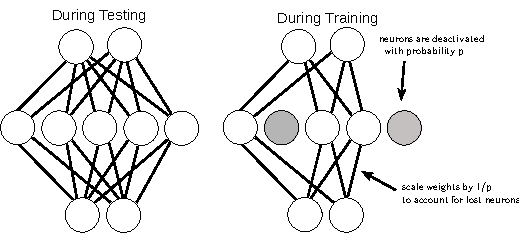
\includegraphics[width=\textwidth]{illustrations/dropout.pdf}
       \captionof{figure}{An illustration of the dropout method. The final network represents
       a possible neural network of 2 input neurons, 5 hidden neurons and 2 output neurons.
       During the training the network becomes thinned via the dropout, different neurons
       are deactivated for each training batch.}
      \end{figure}

    \subsubsection{Early Stopping}
      Early stopping is a form of regularisation where training is stopped early
      to avoid overfitting to the train set (for example, memorisation of examples via high valued weights).
      Often by tracking the losses on
      a validation set an ideal moment to stop can be found \cite{Prechelt2012a}.
\section{Model Evaluation} \label{sec:eval}
  With any kind of classification model it is crucial to be able to evaluate its
  performance in a standard and reproducible way. For the problem of classifying
  AUs the simplest case is to split the problem into a set of $n_C$ decision problems
  where $n_C$ is the number of distinct classes. Now the problem is reduced to
  evaluating the performance of a binary classifier.

  \subsection{Recall, Precision and F1}
    Naively the first metric one might use for measuring the performance of a classifier
    might be the accuracy, this is good for datasets which are evenly balanced however
    the datasets of interest in this report typically have many more negative labels than positive labels.
    A classifier that simply labels all examples negative might then get a very high accuracy. This motivates
    defining a matrix called the confusion matrix whose elements express accuracy from various angles.
    For a binary problem the confusion matrix is defined as:
    \begin{equation}
      C =
      \begin{pmatrix}
        TP & FN\\
        FP & TN
      \end{pmatrix}
    \end{equation}
    Where $TP$ is the number of true positives, $FN$ is the number of false negatives
    , $FP$ is the number of true positives and $TN$ is the number of true negatives.
    In a perfect classification, this matrix would have $FP=FN=0$, however this is
    difficult to achieve
    and we can define quantities to measure how close to this ideal we are. Note we
    only define the binary case here, the more general confusion matrix for multiple
    classes can easily be defined but is not relevant here.
    \begin{equation}
      \text{Recall} = \frac{TP}{TP+FN}
    \end{equation}
    \begin{equation}
      \text{Precision} = \frac{TP}{TP+FP}
    \end{equation}
    \begin{equation}
      \text{F1} = 2 \cdot \frac{\text{Recall} \cdot \text{Precision}}{\text{Recall} + \text{Precision}}
    \end{equation}

    Hence recall is decreased by false negatives, i.e not being able to recall the class
    when presented with it. Precision is decreased by false positives i.e stating the class
    is present when it is not. Both measures describe a different aspect of the accuracy. This
    motivates defining the F1 score which is the harmonic mean between the precision and recall
    (the harmonic mean is used to ensure that case where $R=1$ and $P=0$ R,P being Recall and Precision, gives
    a very low score  as achieving $R=1$ is trivial.) The F1 is the quantity this report will seek to maximise and use to compare
    results with the literature.
  \subsection{Receiver Operating Characteristics}
    Another useful measure is the area under the Receiver operating characteristic (ROC) curve.
    As neural networks output a number between 0 and 1, a threshold must be chosen to signify
    when the network declares a class present. By varying this threshold a series of true positive and false positive rate points
    can be generated, this is the ROC curve. The area under this is ideally 1 and in the worst case 0.5 (TP = FP), hence this is
    another measure of classification accuracy that is invariant to the chosen threshold.

    \begin{table}[]
      \centering \caption{A simple qualitative illustration of what a ROC score means for a classifier.
      Note: It is typically only in strange cases that $ROC< 0.5$ but is possible.} \label{my-lasfasffffabel}
      \begin{tabular}{rl}
        \hline
        Range & Classifier quality \\ \hline
        $0 \leq ROC \leq 0.6$   & Fail               \\
        $0.6 \leq ROC    < 0.7$   & Poor               \\
        $0.7 \leq ROC    < 0.8$   & Fair               \\
        $0.8 \leq ROC    < 0.9$   & Good               \\
        $0.9 \leq ROC \leq 1.0$   & Great              \\ \hline
      \end{tabular}
  \end{table}
  \section{Deep learning approaches to AU detection}
    It has been shown that deep neural networks containing convolutional, max pooling,
    dropout and fully connected layers can effectively learn how to classify AUs in
    a selection of datasets even when ignoring the temporal structure of the data \cite{Gudi2015,Ghosh2015,Khorrami2015}.
    Using the temporal data is also a possibily \cite{emonet,Jaiswal2016}.
    %
    %
    %
    \subsection*{Comparison of networks in Table \ref{tab:compnet}}
    Network \cite{Ghosh2015} (Ghosh et al.) was trained on CK+, DISFA and BP4D datasets.
    A key result of this paper was that they achieved good generalisation between datasets
    with classifications accuracies between 60\% and 80\% for these generalisation experiments.
    A feature particular to this network was that after the softmax layer, which assigns probabilities
    to each AU it uses QDA (Quadratic Discriminant Analysis\cite{precogbook})  to
    make predictions about whether AUs are present. A point of interest is also that
    mean face normalisation is done per subject and then all for all subjects.

    Network \cite{Gudi2015} (Amogh Gudi et al.) was trained on BP4D and SEMAINE
    datasets achieving an average F1 score of 0.52 and 0.34 respectively. This paper
    uses minimal preprocessing hence is a good example of how CNNs can learn features
    with little feature engineering.

    Network \cite{Khorrami2015} (Pooya Khorrami et al.) was trained on TFD and CK+,
    this got average accuracies of 89.9\% and 98.3\% respectively in detecting emotions. This
    is therefore not directly comparable, but they do explore connecting it with AUs.
    An interesting point about this work is that they could stimulate activations in the convolutional
    layers and directly see that the network had learned different facial actions demonstrating the
    power of these networks.

    Network \cite{Jaiswal2016} (Shashank Jaiswal et al.) was trained on SEMAINE and
    BP4D achieving an overall weighted F1 score of 0.54. Which is on average higher
    than network \cite{Gudi2015}. A BLSTM (a recurrent neural network) is used to incorporate temporal structure
    and it defines multiple input streams from each facial region, allowing the convolutional
    filters to become more specialised. This is the only paper where they say they use
    two outputs for each AU so that the softmax creates a probability distribution for
    each AU and not for all of them at once.

    \begin{table}[h!]
    \centering
    \begin{tabular}{lcccc}
    \hline
    Dataset    & \multicolumn{1}{l}{Ghosh et. al\cite{Ghosh2015}} & \multicolumn{1}{l}{Gudi et. al.\cite{Gudi2015}} & \multicolumn{1}{l}{Khorrami et. al.\cite{Khorrami2015}} & \multicolumn{1}{l}{Jaiswal et. al.\cite{Jaiswal2016}} \\ \hline
    CK+      & \checkmark                            &                                      &                                         & \checkmark                              \\
    DISFA    & \checkmark                            &                                      &                                         &                                         \\
    SEMAINE* &                                       & \checkmark                           & \checkmark                              &                                         \\
    BP4D*    & \checkmark                            & \checkmark                           & \checkmark                              &                                         \\
    TFD      &                                       &                                      &                                         & \checkmark                              \\ \hline
    \end{tabular}
    \caption{A comparison of which datasets were used in the relevant papers.} \label{compdat}
    \end{table}

    It should be noted that it is difficult to compare the performance between these
    networks as they all use different evaluation scores as shown in table \ref{compscore}. Table \ref{compdat} also shows
    which datasets each of the discussed papers used.
    \begin{landscape}
    \begin{table}[h!]
    % \centering
    {\footnotesize
    \begin{tabular}{|lllllllll|}
    \hline
    Network                      & \multicolumn{2}{c}{Ghosh et. al\cite{Ghosh2015}}                         & \multicolumn{2}{c}{Gudi et. al.\cite{Gudi2015}}                            & \multicolumn{2}{c}{Khorrami et. al.\cite{Khorrami2015}}                          & \multicolumn{2}{c|}{Jaiswal et. al.\cite{Jaiswal2016}}   \\ \hline
    \multicolumn{1}{|l|}{Element} & Type     & \multicolumn{1}{l|}{Dimensions}                    & Type     & \multicolumn{1}{l|}{Dimensions}                      & Type          & \multicolumn{1}{l|}{Dimensions}                  & Type      & Dimensions                     \\ \hline
    \multicolumn{1}{|l|}{x}       &          & \multicolumn{1}{l|}{$40\times40\times1$}           &          & \multicolumn{1}{l|}{$48\times 48\times1$}            &               & \multicolumn{1}{l|}{$96\times96\times1$}         &           & $?\times?\times1$              \\ \hline
    \multicolumn{1}{|l|}{$L_1$}   & conv 1   & \multicolumn{1}{l|}{$12\times 12\times1\times 70$} & conv 1   & \multicolumn{1}{l|}{$5\times 5\times1\times64$}      & conv 1        & \multicolumn{1}{l|}{$5\times5\times1\times64$}   & conv 1*   & $5\times5\times(2n+1)\times32$ \\
    \multicolumn{1}{|l|}{$y_1$}   &          & \multicolumn{1}{l|}{$29\times29\times70$}          &          & \multicolumn{1}{l|}{$44\times44\times64$}            &               & \multicolumn{1}{l|}{$92\times92\times64$}        &           & $?\times?\times32$             \\ \hline
    \multicolumn{1}{|l|}{$L_2$}   & max pool & \multicolumn{1}{l|}{$2\times 2$}                   & max pool & \multicolumn{1}{l|}{$3\times3$ (stride 2)}           & max pool      & \multicolumn{1}{l|}{$2\times2$}                  & max pool*  & $3\times3$                    \\
    \multicolumn{1}{|l|}{$y_2$}   &          & \multicolumn{1}{l|}{$15\times15\times 70$}         &          & \multicolumn{1}{l|}{$22\times 22\times64$}           &               & \multicolumn{1}{l|}{$46\times46\times64$}        &           & $?\times?\times32$             \\ \hline
    \multicolumn{1}{|l|}{$L_3$}   & conv 2   & \multicolumn{1}{l|}{$4\times 4\times70\times 10$}  & conv 2   & \multicolumn{1}{l|}{$5 \times 5 \times 64\times64$}  & conv 2        & \multicolumn{1}{l|}{$5\times5\times64\times128$} & conv 2    & $5\times5\times32\times64$     \\
    \multicolumn{1}{|l|}{$y_3$}   &          & \multicolumn{1}{l|}{$12\times 12 \times 10$}       &          & \multicolumn{1}{l|}{$18 \times 18\times64$}          &               & \multicolumn{1}{l|}{$42\times42\times128$}       &           & $?\times?\times64$             \\ \hline
    \multicolumn{1}{|l|}{$L_4$}   & max pool & \multicolumn{1}{l|}{$2\times 2$}                   & conv 3   & \multicolumn{1}{l|}{$4\times 4 \times64 \times 128$} & max pool      & \multicolumn{1}{l|}{$2\times2$}                  & conv 3    & $5\times5\times64\times64$     \\
    \multicolumn{1}{|l|}{$y_4$}   &          & \multicolumn{1}{l|}{$6\times 6 \times 12$}         &          & \multicolumn{1}{l|}{$15\times15\times128$}           &               & \multicolumn{1}{l|}{$21\times21\times128$}       &           & $?\times?\times64$             \\ \hline
    \multicolumn{1}{|l|}{$L_5$}   & fc       & \multicolumn{1}{l|}{$500$}                         & fc       & \multicolumn{1}{l|}{$3072$}                          & conv 3        & \multicolumn{1}{l|}{$5\times5\times1\times256$}  & conv 3    & $4\times4\times64\times128$    \\
    \multicolumn{1}{|l|}{$y_5$}   &          & \multicolumn{1}{l|}{$500$}                         &          & \multicolumn{1}{l|}{$3072$}                          &               & \multicolumn{1}{l|}{$17\times17\times256$}       &           & $?\times?\times128$            \\ \hline
    \multicolumn{1}{|l|}{$L_6$}   & fc       & \multicolumn{1}{l|}{$100$}                         & softmax  & \multicolumn{1}{l|}{$12$}                            & quadrant pool & \multicolumn{1}{l|}{}                            & fc        & $3072$                         \\
    \multicolumn{1}{|l|}{$y_6$}   &          & \multicolumn{1}{l|}{$100$}                         &          & \multicolumn{1}{l|}{$12$}                            &               & \multicolumn{1}{l|}{$4\times4\times256$}         &           & $3072$                         \\ \hline
    \multicolumn{1}{|l|}{$L_7$}   & softmax  & \multicolumn{1}{l|}{$12$}                          &          & \multicolumn{1}{l|}{}                                & fc            & \multicolumn{1}{l|}{$300$}                       & softmax   & $2N_{C}$                       \\
    \multicolumn{1}{|l|}{$y_7$}   &          & \multicolumn{1}{l|}{$12$}                          &          & \multicolumn{1}{l|}{}                                &               & \multicolumn{1}{l|}{$300$}                       &           & $2N_{C}$                       \\ \hline
    \multicolumn{1}{|l|}{$L_8$}   & QDA      & \multicolumn{1}{l|}{}                              &          & \multicolumn{1}{l|}{}                                & softmax       & \multicolumn{1}{l|}{$8$}                         & BLSTM     &                                \\
    \multicolumn{1}{|l|}{$y_8$}   &          & \multicolumn{1}{l|}{}                              &          & \multicolumn{1}{l|}{}                                &               & \multicolumn{1}{l|}{$8$}                         &           &                                \\ \hline
    \end{tabular}

    \caption{A comparison of network architectures from the literature, all networks
    use RELUs as their activation functions apart from in the final layer where it is
    typical to use a softmax. $x$ denotes the input image, $L_i$ denotes the $i$th layer and $y_i$ denotes the output of the $i$th layer.
    $N_{C}$ is the number of classes.
    The question marks signify the dimensions of input images are variable as it depends on the input stream. fc is for fully connected and
    conv is for a convolutional layer. QDA is Quadratic Discriminant Analysis and BLSTM is for Bidirectional Long Short-Term Memory neural
    networks.
    \newline
    *These layers are per input stream} \label{tab:compnet}

    }
    \end{table}
    \begin{table}[h!]
    \centering
    \begin{tabular}{lcccc}
    \hline
    Score    & \multicolumn{1}{l}{Ghosh et. al\cite{Ghosh2015}} & \multicolumn{1}{l}{Gudi et. al.\cite{Gudi2015}} & \multicolumn{1}{l}{Khorrami et. al.\cite{Khorrami2015}} & \multicolumn{1}{l}{Jaiswal et. al.\cite{Jaiswal2016}} \\ \hline
    Accuracy & \checkmark                                       &                                                 & \checkmark                                             &                                             \\
    F1       &                                                  & \checkmark                                      &                                                        & \checkmark                                  \\
    AUC     & \checkmark                                       & \checkmark                                      &                                                        &                                             \\ \hline
    \end{tabular}
    \caption{A comparison of which evaluation methods were used in the relevant papers.} \label{compscore}
    \end{table}
    \end{landscape}
